% !TEX root = writing_version.tex

\label{chp:data_analysis}
\section{Parameter choice of the simulated system}
\label{sec:system_choice}
As an integral part of this work large scale simulations have been executed on the NEMO High performance computation (HPC) cluster. The input parameters of the simulated systems are given in \autoref{tab:system_1m}.

\begin{table}[ht]
\centering
\begin{tabular}{c|c}
Parameter & Value \\ \hline
N & 1048576 \\
eq\_steps/particle & 1000 \\
pr\_steps/particle & 20000  ... 60000 \\
$\eta_i$ & 45.0 \% \\
$\eta_f$ & 53.1\% ... 53.4 \% \\
\end{tabular}
\caption[Simulation parameters of data production systems]{Input parameters of large scale simulations on the NEMO HPC cluster. The varying steps during production come by the fact, that 20000 steps were estimated to be calculated within 3 days leaving 1 day of buffer to the hard wall time limit of 4 days. Due to the increasing calculation cost of the q6q6 cluster routines for large clusters the wall time limit was still breached and without proper reset steps the datasets could not be restarted without large calculation overhead as all lost data has to be replaced, and the broken reset steps within the files would have to be removed prior to further simulations. Therefore the last proper version of the files were used resulting in varying simulation lengths but only rarely without nucleation event in the case of early breakdown.}
\label{tab:system_1m}
\end{table}

The simulations comprise four series' at volume fractions of $\eta = 0.531,\;0.532,\;0.533 \text{ and }0.534$ where each series consists of 500 trajectories. Therefore at each volume fraction a total number of about half a billion particles have been simulated in the metastable fluid.\\

The volume fractions have been chosen to probe nucleation rates to the lowest possible limit. As single nucleations have been observed down to volume fractions of $\eta=53.2\%$, the lowest volume fraction was set to just below this value as the large statistic of 500 trajectories was expected to still yield enough nucleation events to measure their rate.\\

The size of the systems was chosen comparably large with about 1 million particles. These large systems intuitively seem to be in conflict with the long induction times, but using CNT as a guideline it can be shown that the computational effort for simulating nucleation events does not increase significantly with increasing system size. As the calculation time per unit of simulation time is proportional to N, it is at a given volume fraction also proportional to the volume V:
\begin{align}
\label{eqn:system_size}
\frac{T_{CPU}}{\delta t_{Sim}} \propto N \propto V 
\end{align}

Further we expect the nucleation time in terms of the system time $\langle \tau_{Nucleation} \rangle$ to be proportional to the inverse of the system volume if assuming a nucleation rate density independent of time:
\begin{align}
\langle \tau_{Nucleation} \rangle \propto \frac{1}{V}
\end{align}

As the required CPU time for a nulcleation event is simply proportional to the product of $\langle \tau_{Nucleation} \rangle$ and the calculation time per unit of system time we can conclude:

\begin{align}
\langle T_{CPU} \rangle \propto  \frac{T_{CPU}}{\delta t_{Sim}}  \cdot \langle \tau_{Nucleation} \rangle \propto \frac{V}{V} = \text{const.}
\end{align}

Thus the size of the system is only relevant to be chosen smaller if ordering processes are important for the system, as the initial induction time would be independent of the system size. This might be the case for polydisperse systems, but in the monodisperse case the above reasoning was found to hold true.\\
An other objective that has to be considered is that less configuration snapshots of the system can be stored, as these requrie a lot of memory space. If one is interested in quantites like $g(r)$ this is not a problem as the necessary statistics can be either derived from a large set of small snapshot or from a small set of large snapshots, but for example resolving and storing the dynamcs of a configuration for a growing cluster would require using smaller system sizes as files easily grow to many GB's in size. 

\section{Long time diffusion time scale}
\label{sec:diffusion_metastable_liquid}
Diffusion or more precisely self-diffusion, characterizes the movement of the single particles within the system. While the diffusive behavior often can be subdivided into different regimes with different physical meanings as discussed in \autoref{sec:diffusion_probe}, only the long time diffusion constant is measured for the hard sphere system. To circumvent finite size effects we use unwrapped coordinates in which case the long time movement of the particles is governed by the relation \autoref{eqn:einstein_relation} which was first described by Einstein 1905\cite{Albert1905}.

\begin{align}
\label{eqn:einstein_relation}
D^S_L = \underset{t\rightarrow \infty}{\text{lim}} \frac{\langle (\vec{r}(t) - \vec{r}(0) )^2 \rangle}{2 d t}
\end{align}

With $D^S_L$ the long time self-diffusion constant which will in the following be denoted only by $D_L$, $\vec{r}(t)$ the position of a particle at time t, d the number of spatial dimensions of the system and $\langle ... \rangle$ the expectation value of the ensemble.\\

The average is measured by saving a reference position of all particles at one point, and furthermore carrying a set of unwrapped positions through the simulation. The squared distance between reference position and unwrapped position is averaged over all particles and used as the measurement of the ensemble average. Especially for large system of 1 million particles, this quantity has only very small fluctuations as can be seen in \autoref{fig:diffusion_comparison}, where the slopes of the linear regressions to the MSD trajectories are depicted.\\

\begin{figure}[ht]
\begin{center}
\subfloat[Histograms of the slopes for the linear regressions to the mean squared displacements. The histograms are for $\eta=0.531,\;0.532,\;0.533,\;0.534$.]{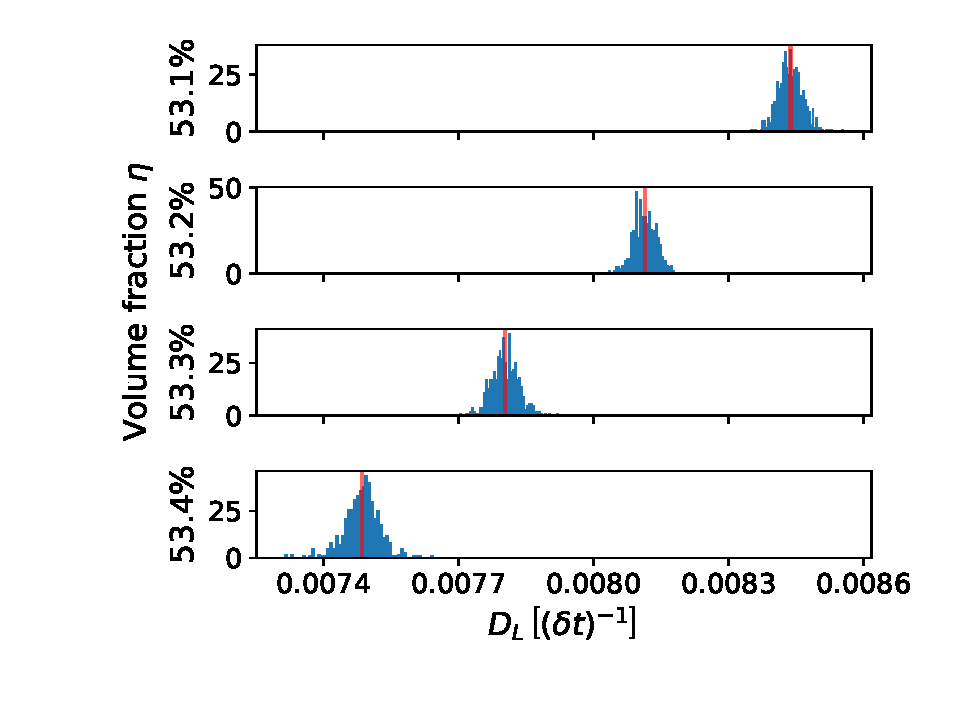
\includegraphics[width = 0.45 \textwidth]{diffusion_histogram_comparison.pdf}} \hspace{0.5cm}
\subfloat[Mean of the histograms with the uncertainty on the mean given by $\sigma_{\langle D_L \rangle} = \sigma_{D_L}/\sqrt{n}$ with n being the number of measurements included in the average.]{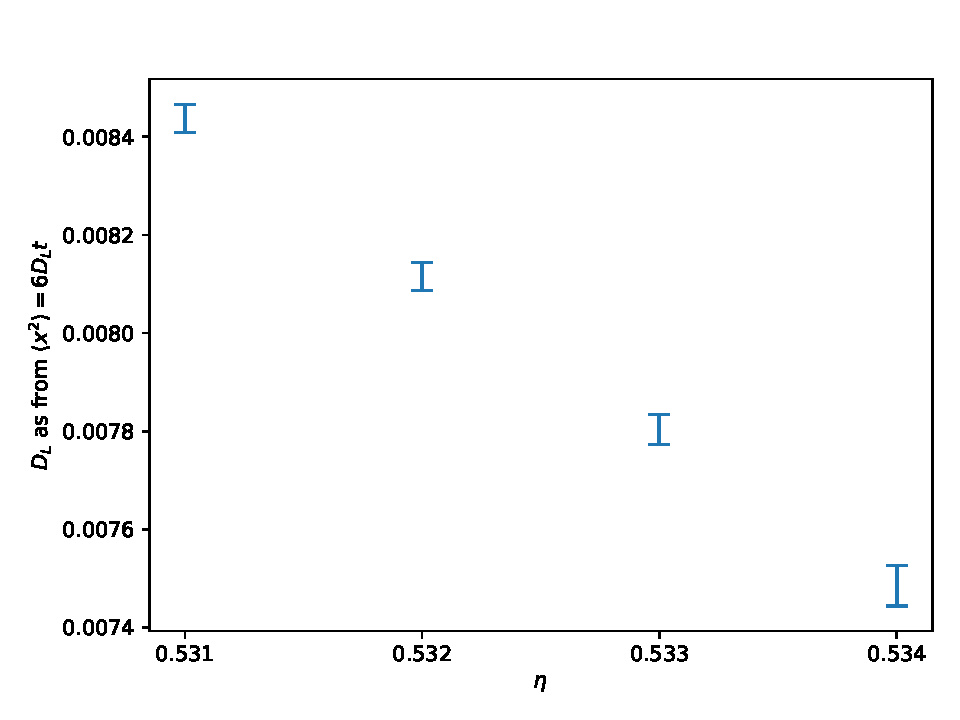
\includegraphics[width = 0.45 \textwidth]{diffusion_comparison.pdf}}  
\caption[Long time self-diffusion constant measurements from production data]{Comparison of long time self-diffusion constants at different volume fractions as histograms and means with uncertainty. As we see the }
\label{fig:diffusion_comparison}
\end{center}
\end{figure}

The diffusion coefficients are used to make the time scales of different experiments comparable. It is based on the idea that the fundamental mechanisms for nucleation and cluster growth do not vary between different hard sphere like systems, but are only scaled by the varying diffusion times. Furthermore there are theoretical predictions for the relationship of short time and long time diffusion, making it possible to compare experiments where the short time diffusion behavior is better accessible with the ballistic simulations where only the long time diffusion constant is measurable.\\


As we see in \autoref{fig:diffusion_comparison} the diffusion constants can be measured at high precision with a relative standard deviation of $\sigma_{D_L}/D_L \approx 1\%$. Hence it does not introduce large uncertainties when normalizing time related quantities by the diffusion time $\tau_{D_L} = D_L^{-1}$.

\section{Cluster size distribution over time}
\label{sec:pnt}
The cluster size distribution of the system can be used to test the assumption of Markovian dynamics by trying to find a Fokker-Planck equation describing the time evoluation of the distribution. This has been done for the Lennard-Jones system by Kuhnbold et al. 2019\cite{Kuhnbold2019}. Testing the trajectories shown in \autoref{fig:pnt_short} and \autoref{fig:pnt_long} in a similar fashion would yield a good comparison but due to time constraints of this thesis it is not done. We still can illustrate some characteristics of the metastable fluid directly after and long after the quench as it compactly shows some main features of the systems behavior.\\ 

The cluster size distributions are the averages over all trajectories at a given volume fraction. While they are normalized by the number of included measurements they have not been normalized by the volume. The maximum cluster size is set to 160 as above this value only nucleating trajectories can be seen. Also a logarithm to the base of 10 is used, and cluster sizes not present at a given time step have been fixed to a value below the minimal signal as the logarithm requires non zero values.\\
The logarithm is used because the mesurements span orders of magnitude and further it then can be interpreted as a quantity proportional to a free energy. This is justified by assuming that the cluster size distributions represents the correpsonding probability distribution and that stationary states may fluctuate in a free energy landscape where the probability for a particular state with some energy $\Delta E$ is given by a Boltzmann distribution $p\propto \exp \left( - \frac{\Delta E}{k_B T} \right)$ from which follows that $\log(p) \propto \Delta E$.\\

\begin{figure}[ht]
\begin{center}
\subfloat[$\eta = 53.1\%$]{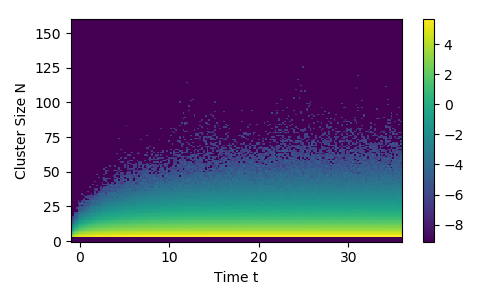
\includegraphics[width = 0.49 \textwidth]{pnt_531_short.png}} \hspace{0.0cm}
\subfloat[$\eta = 53.2\%$]{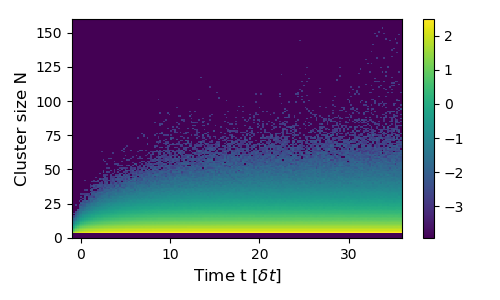
\includegraphics[width = 0.49 \textwidth]{pnt_532_short.png}}\\
\subfloat[$\eta = 53.3\%$]{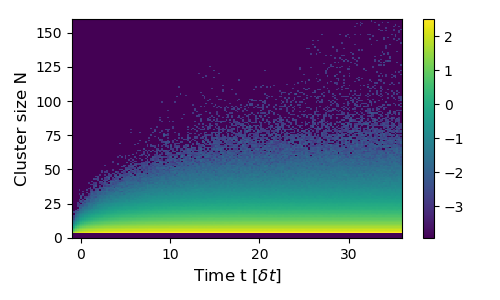
\includegraphics[width = 0.49 \textwidth]{pnt_533_short.png}} \hspace{0.0cm}
\subfloat[$\eta = 53.4\%$]{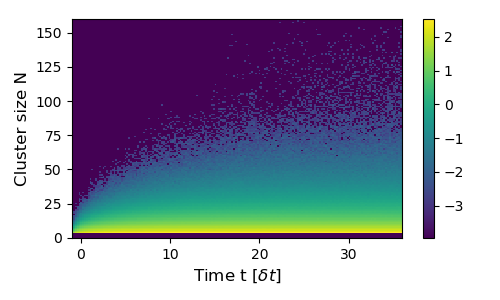
\includegraphics[width = 0.49 \textwidth]{pnt_534_short.png}}
\caption[Cluster size distributions over time after quench]{Decadic logarithm of cluster size distributions for different volume fractions in the initial phase after the quench.}
\label{fig:pnt_short}
\end{center}
\end{figure}

In \autoref{fig:pnt_short} we can see the initial phase after the quench. As the fluid before the quench was at a volume fraction of $\eta=45\%$ only very little local ordering is present directly after the quench. This changes within the first $15 -25 \delta t$ after which the distribution becomes stable, where the exact length depends on the volume fraction. This might be explained by assuming that the initial phase is how long it takes for the system to build up the local ordering in the metastable liquid and as the clusters tend to be larger for higher volume fractions more particles are required to find their ordering.\\   
To further compare the system time with the more intuitive number of collisions per particle we can use that at the given volume fraction we find  $1\delta t \approx \frac{60 events}{particle}$. When further using a collision probability of $\sim 40 \%$ for each executed event, we find that $1\delta t \approx \frac{25 collisions}{particle}$. As a result we can conclude that it takes a few hundred collisions for each particle to build up the local ordering with unstable clusters.\\

\begin{figure}[ht]
\begin{center}
\subfloat[$\eta = 53.1\%$]{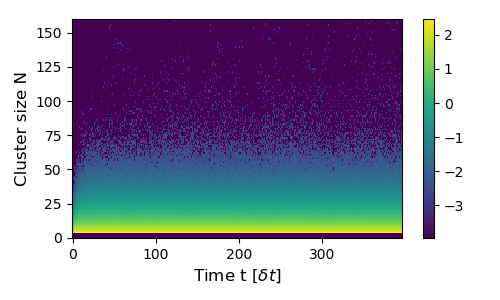
\includegraphics[width = 0.49 \textwidth]{pnt_531_long.png}} \hspace{0.0cm}
\subfloat[$\eta = 53.2\%$]{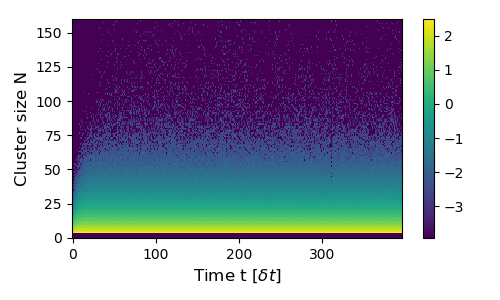
\includegraphics[width = 0.49 \textwidth]{pnt_532_long.png}}\\
\subfloat[$\eta = 53.3\%$]{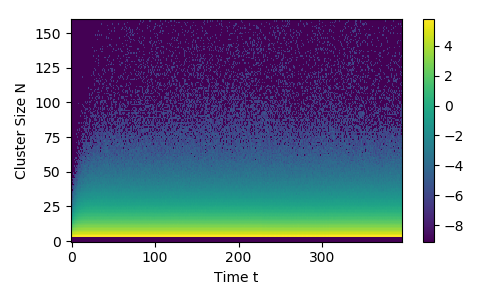
\includegraphics[width = 0.49 \textwidth]{pnt_533_long.png}} \hspace{0.0cm}
\subfloat[$\eta = 53.4\%$]{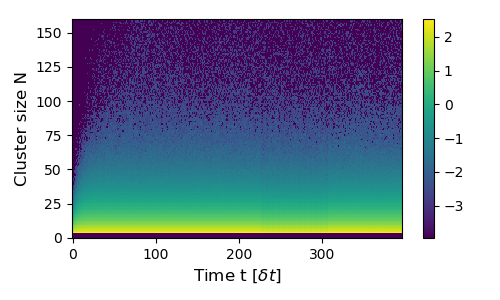
\includegraphics[width = 0.49 \textwidth]{pnt_534_long.png}}
\caption[Cluster size distributions for long waiting times]{Decadic logarithm of cluster size distributions for different volume fractions during the waiting time.}
\label{fig:pnt_long}
\end{center}
\end{figure}

The diagrams in \autoref{fig:pnt_long} show a zoomed out version of the same data depicted already in \autoref{fig:pnt_short}. We see that the distribution that is reached at the end of the initial phase remains stable over prolonged periods of time. Only the nulceation events which account for most of the probability at largest cluster sizes indicate that this is not a stable process but only a metastable one. Nevertheless this does not mean that it simply can be viewed as a stationary process, because when taking the ensemble as a whole, at any point of time phase transitions take place at various parts of the system.

\section{Autocovariance functions of largest cluster in the metastable fluid}
\label{sec:acf}
The autocovariance function (ACF) of the largest cluster contains information about how long a single cluster persists as the largest cluster within the volume. This is because fluctuations of clusters at different points of the volume are expected to be independent of each other and only the size of a distinct cluster should be correlated in time.\\

The autocovariance function is defined by \autoref{eqn:definition_acf} where $N_{\text{lc}}(t)$ is the number of particles in the largest cluster at time t, $\langle N_{\text{lc}} \rangle_t$ is the corresponding average over time and thus $X(t)$ describes the deviations from the average. The autocovariance function furthermore is normalized by ${ \langle X^2  \rangle }$, the variance of the data, such that $ACF(0) = 1 $.

\begin{align}
\label{eqn:definition_acf} 
ACF(\tau)=\frac{ \langle  X(\tau) \cdot  X(0) \! \: \rangle }{ \langle X^2  \rangle }\\  
\text{with } X(t)=N_{\text{lc}}(t)- \langle N_{\text{lc}} \rangle_t 
\end{align}

The ACF is calculated from the largest cluster measurement for each trajectory. Because after a nucleation event the largest cluster size surely is correlated in time, only those parts of the measurements that did not involve strong cluster growth are used. Therefore the ACF's in \autoref{fig:acf} show the temporal correlations of the largest cluster in the metastable fluid.\\

\begin{figure}[ht]
\begin{center}
\subfloat[$\eta = 0.531$]{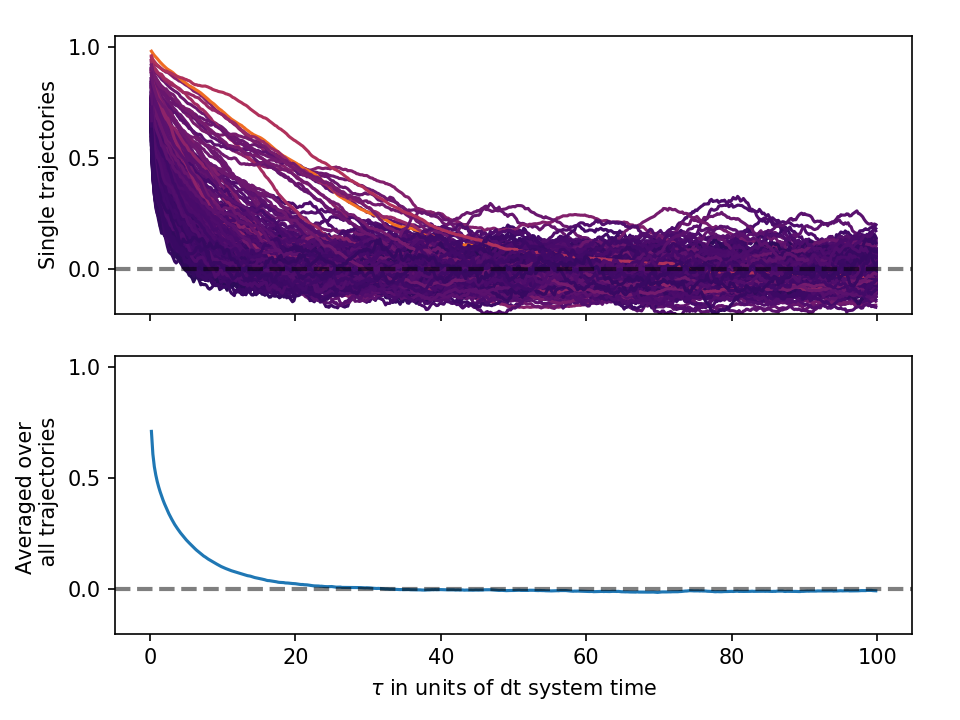
\includegraphics[width = 0.4 \textwidth]{acf_lc_531.png}} \hspace{0.5cm}
\subfloat[$\eta = 0.532$]{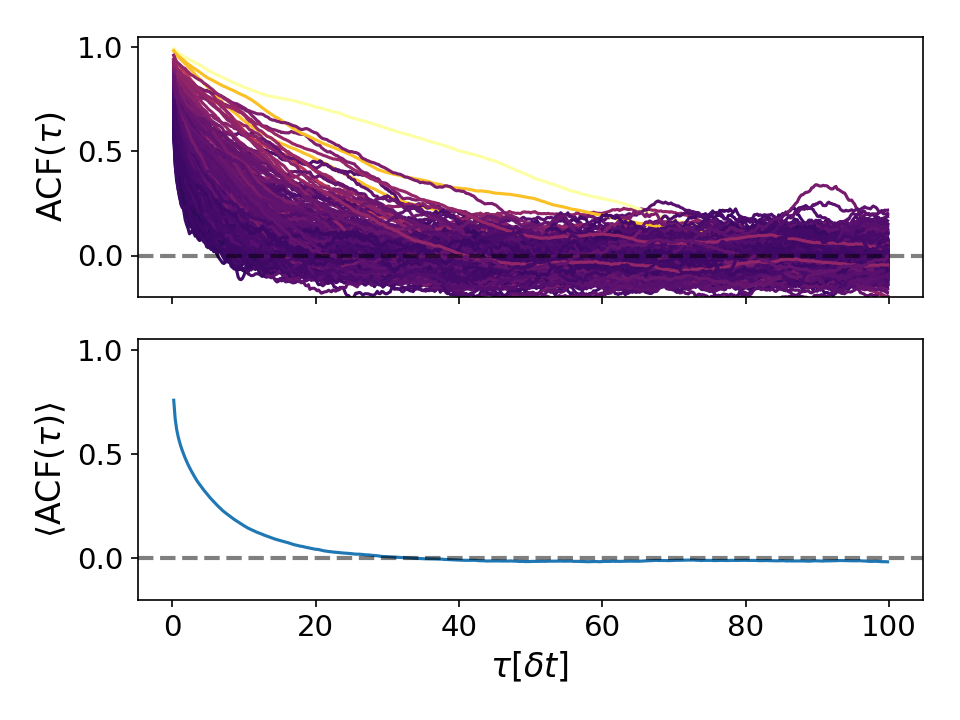
\includegraphics[width = 0.4 \textwidth]{acf_lc_532.png}} \\
\subfloat[$\eta = 0.533$]{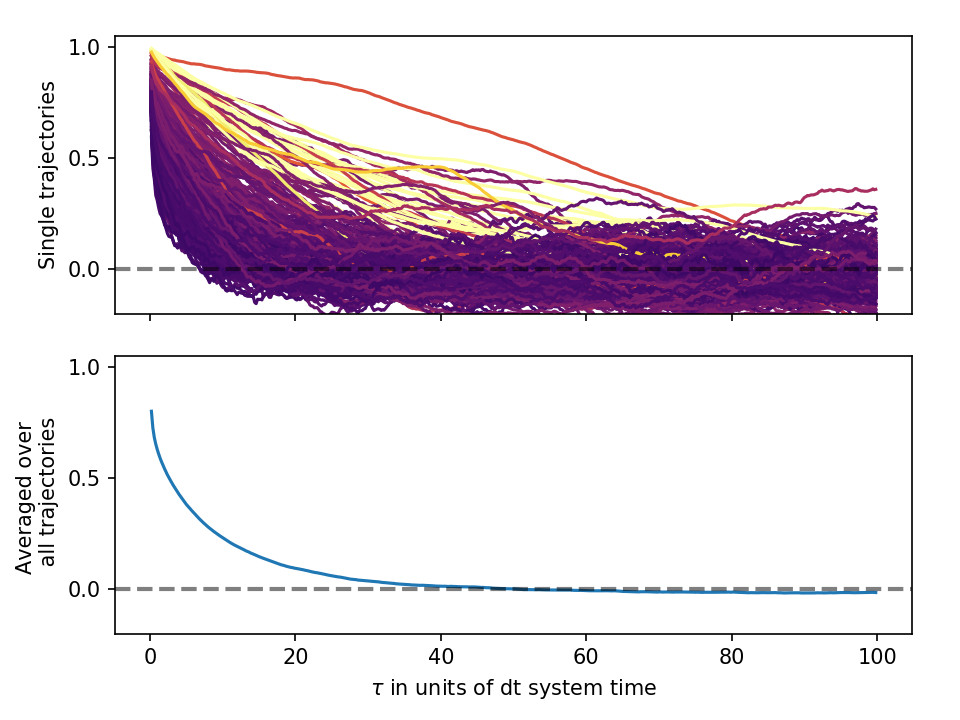
\includegraphics[width = 0.4 \textwidth]{acf_lc_533.png}} \hspace{0.5cm}
\subfloat[$\eta = 0.534$]{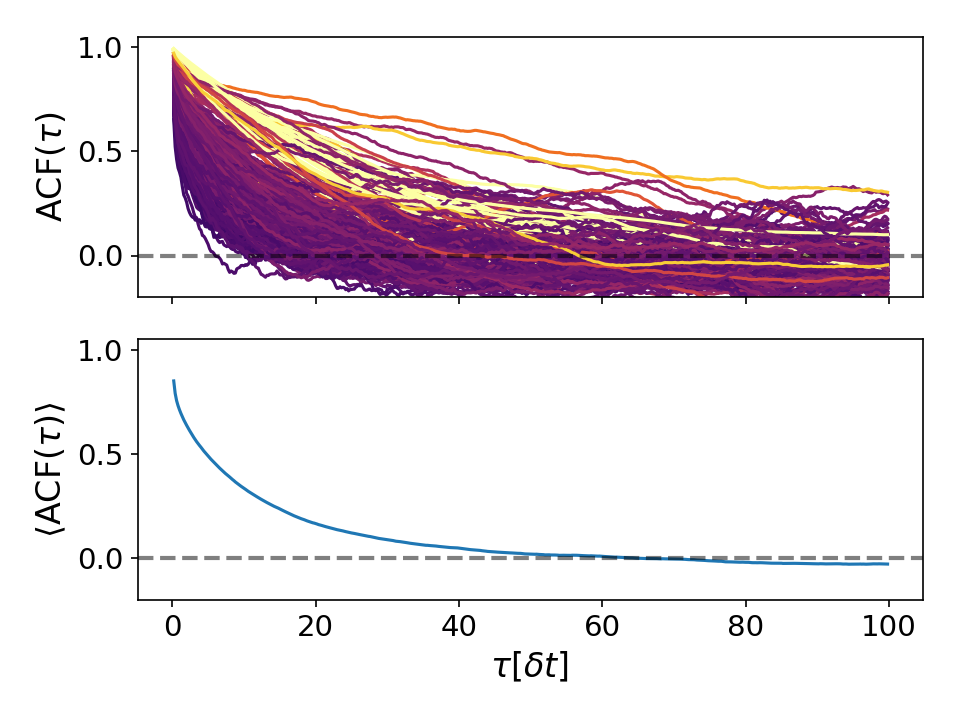
\includegraphics[width = 0.4 \textwidth]{acf_lc_534.png}} \\
\caption[Autocovariance functions of largest cluster in the metastable fluid]{Comparison of autocovariance functions in the metastable fluid. The top of each diagram depicts all trajectories with coloring for the largest cluster size within the used time interval. The lightest color thereby indicates a largest cluster of more than 500 hundred particles which is a nucleation event. As these are rare in the given selection, the data represents the metastable fluid well. The bottom of each diagram shows the average of the above one with decay times of $ 15 \delta t- 35 \delta t$ depending on the volume fraction. }
\label{fig:acf}
\end{center}
\end{figure}

The decay of the autocovariance functions indicates that structural fluctuations persist for longer times at higher volume fractions. From the coloring, that corresponds to the maximum cluster size within the trajectory, we can also conclude that the fluctuations tend to be larger at higher volume fractions and that for $\eta=53.4\%$ a signal from nucleation events might not be completly negligible anymore. The larger mestastable clusters were also seen before in the cluster size distributions in \autoref{sec:pnt}.\\
The time scale on which the ACF decays corresponds closely to the initial ordering time observed for the cluster distribution directly after the quench. Furthermore it also correpsonds to the lifetimes of large clusters found in the single example of the individual cluster tracking algorithm (\autoref{fig:lifetime}). This leads to the conclusion that these three observations all show the same time scale of local ordering processes within the metastable fluid. 

\section{Cluster growth and constant attachement rate}
\label{sec:cluster_growth}
Once the clusters reach a certain size they are expected to grow with new particles being attached to the surface at a constant rate leading to a growth with a proportionality of $N \propto t^3$ as shown in \autoref{eqn:constant_growth}, with k being the constant attachment rate, N the number of particles in a specific cluster, A the surface of the cluster, R the radius of the cluster and $\rho_{solid}$ the bulk density which for large clusters is a good approximation of the cluster density.\\
\begin{align}
\label{eqn:constant_growth}  
\begin{split}
\dot{N} &= A k \\
          & \; \; \, \vrule
  \begin{aligned}[t]
    \quad \text{with}  \quad  N &= \frac{4}{3} \pi R^3 \rho_{solid}\\
    \Leftrightarrow R &= \left( \frac{3 N }{4 \pi \rho_{solid} }\right)^{\frac{1}{3}} \, \text{,} \\
    \quad \text{and}   \quad A &= 4 \pi R^2 \\
    \Leftrightarrow A &= \left(\frac{4 \pi 3^2 }{\rho_{solid}^2} \right)^\frac{1}{3} N^\frac{2}{3} \, \text{,}\\
%    \quad \text{follows} \quad A &\propto N^\frac{2}{3} \\
  \end{aligned}\\
\frac{dN}{dt} &= \left(\frac{4 \pi 3^2 }{\rho_{solid}^2} \right)^\frac{1}{3}  N^\frac{2}{3} k \\
\end{split}
\hspace{1cm}
\begin{split}
%\Rightarrow \frac{dN}{dt} &= c' N^\frac{2}{3}\nonumber\\
%\vspace{0.25cm}\nonumber\\
& \!\!\!\!\!\!\!\!\! \text{From the bottom left side}\\
\Rightarrow& \quad dN \; N^{-\frac{2}{3}} = \left(\frac{4 \pi 3^2 }{\rho_{solid}^2} \right)^\frac{1}{3} k \; dt\\
          & \; \; \, \vrule
  \begin{aligned}[t]
    \quad \text{setting}  \quad  N(t=0) = 0\\
  \end{aligned}\\
\Leftrightarrow& \quad 3 N^{\frac{1}{3}} = \left(\frac{4 \pi 3^2 }{\rho_{solid}^2} \right)^\frac{1}{3} k t\\
\Leftrightarrow&  \quad N^{\frac{1}{3}} = \left( \frac{4 \pi}{3 \rho_{solid}^2} \right)^\frac{1}{3} k t
\end{split}
\end{align}  

As the systems are able to accommodate clusters up to a few hundred thousand particles and mostly just one cluster forms during a simulation, the attachment rate can be measured by a linear regression to the third root of the number of particles in the largest cluster over time. As an example this is visualized for the trajectories at $\eta=0.532$ in \autoref{fig:cluster_growth_example}.

\begin{figure}[ht]
\centering
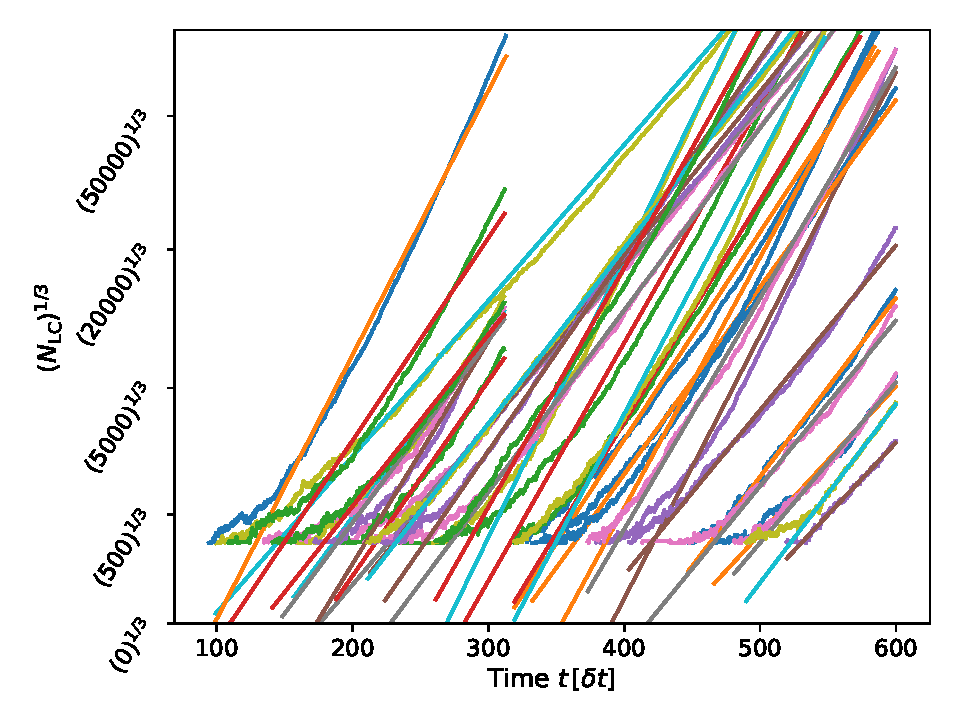
\includegraphics[width=0.7 \linewidth]{cluster_growth_example.pdf}
\caption[Largest cluster trajectories from production data with constant attachment rates]{Trajectories of the third root of the number of particles within the largest cluster $(N_{\text{LC}})^{1/3}$ over time. Clearly visible is the linear proportionality for which a linear regression is shown together with the data. The cut of some data sets at $t \approx 300 \delta t $ is due to the trespassing of the maximum wall time of the NEMO computational cluster. Systems that hosted a nucleation event in the first simulation interval before $T \approx 300\delta t  $, contain a too large cluster in the next simulation interval leading to the breach of the wall time limit due to the quadratic effort required for the q6q6 cluster finding routine. It can be assumed that clusters forming just before $t \approx 300 \delta t$ might not have been recognized due to this flaw. But the number of trajectories concerned by this is small and the impact is not easy to recognize when looking at the induction time distributions in \autoref{fig:induction_distributions}.}
\label{fig:cluster_growth_example}
\end{figure}

Subsequently the slopes of the linear regressions have been collected in histograms shown in \autoref{fig:constant_growth_rates}. By \autoref{eqn:constant_growth} these slopes correspond to constant attachment rates with a prefractor depending on the density within the cluster, but as the densities of concern are very close to each other they only introduce a relative difference of 0.5\% between the rates of lowest and highest volume fractions. For this reason the dependence is neglected in the qualitative comparison and the constant attachement rate with its prefactor is defined as $ c \coloneqq k \left( \frac{4 \pi}{3 \rho_{solid}^2} \right)^\frac{1}{3} $. With this approximation the equation for the number of particles in a cluster over time, given in \autoref{eqn:constant_growth}, simplifies to the one given before in \autoref{eqn:simple_growth}.\\ 

\begin{figure}[ht]
\begin{center}
\subfloat[Histograms of the slopes from the linear regressions to third root of the largest cluster during the stable growth process. The histograms are for $\eta=0.531,\;0.532,\;0.533,\;0.534$.]{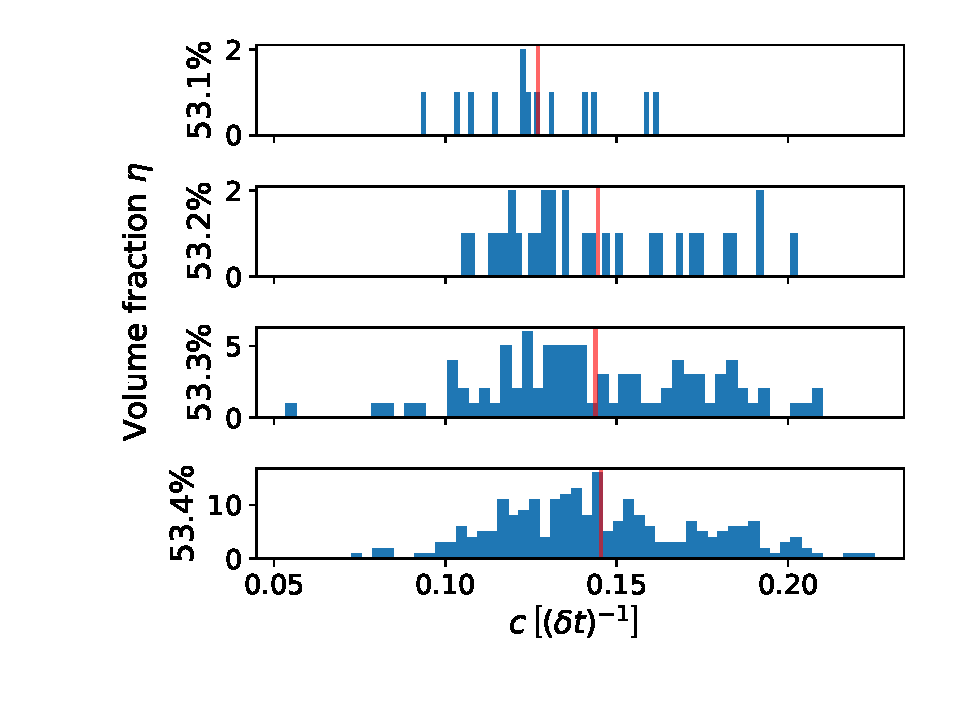
\includegraphics[width = 0.45 \textwidth]{const_growth_rate_histogram_comparison.pdf}} \hspace{0.5cm}
\subfloat[Mean of the histograms with the uncertainty on the mean given by $\sigma_{\langle c \rangle} = \sigma_c/\sqrt{n}$ with n being the number of measurements included in the average.]{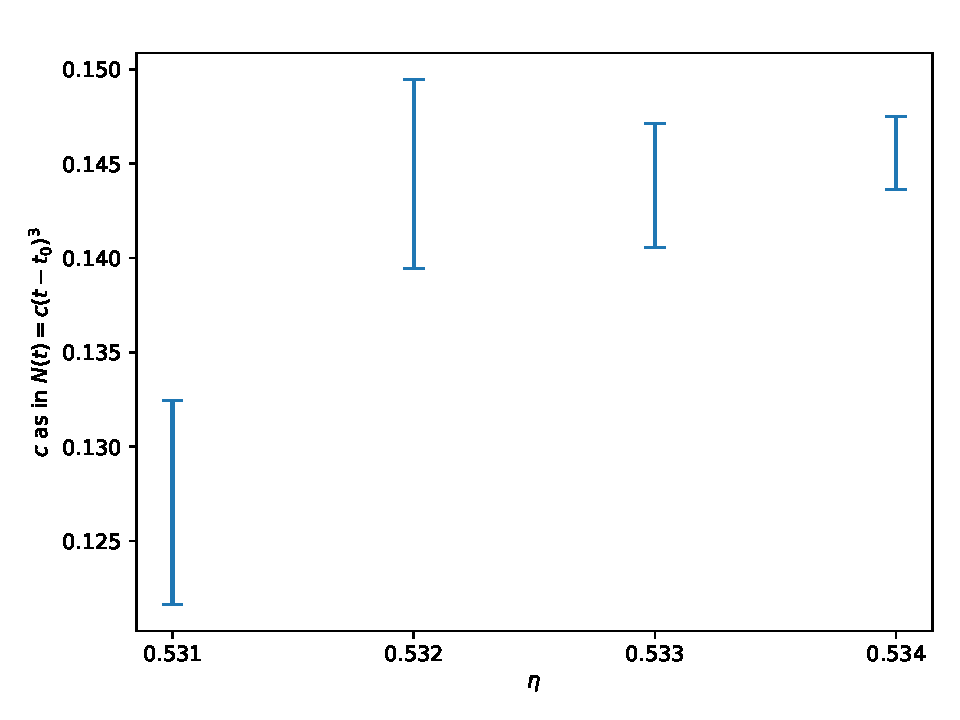
\includegraphics[width = 0.45 \textwidth]{const_growth_rate_comparison.pdf}}  
\caption[Constant attachment rate measurements from production data]{Comparison of growth rates in the constant attachment regime.}
\label{fig:constant_growth_rates}
\end{center}
\end{figure}

What we see from the histograms is that the distribution is rather spread out, but not significantly depending on the volume fraction. Only for $\eta = 0.531$ we find a smaller growth rate. A possible explanation for this behavior could be that the growth by heterogeneous crystallization on the cluster surface leads to a higher growth rate for higher volume fractions as it is less likely for the lower volume fractions. But due to the low statistics at the lowest volume fraction it is also possible that only a statistical fluctuation is seen.\\ 
To investigate if the attachement is diffusion or reaction controlled we may note that the diffusion constants vary from $D=0.0081|_{\eta = 0.532}$ to $D=0.0075|_{\eta = 0.534}$. They span a difference of about 7.5\% but as the relative statistical uncertainty of the growth rates is of the order of 5\% it requires a larger number of samples to answer this question.

\section{Tensor of gyration evaluation}
\label{sec:tog}
The tensor of gyration is a very useful tool as it describes the second moments of the position distributions. Thus it comprises information about the spatial extent in all three dimensions with commonly defined quantities being the radius of gyration, asphericity and anisotropy, see Theodorou and Suter 1985\cite{Theodorou1985}.\\

The tensor of gyration itself is defined by
\begin{align}
\label{eqn:tensor_of_gyration}
&S_{mn}=\frac{1}{N} \sum_{i=1}^{N} r^{(i)}_m r^{(i)}_n\\
\label{eqn:center_of_mass}
&\text{with} \quad \sum_{i=1}^{N} \vec{r}^{(i)} = 0 \; \text{.}
\end{align}

As described by \autoref{eqn:center_of_mass} the matrix $S_{mn}$ is calculated in the center of mass frame for particles with the same mass. The tensor of gyration can be diagonalized, with the three Eigenvalues $\lambda_1^2$, $\lambda_2^2$ and $\lambda_3^2$ that are chosen with $\lambda_1^2 \leq \lambda_2^2 \leq \lambda_3^2 $. These three Eigenvalues correspond to the spatial extents of the cluster within the Cartesian system in which the tensor of gyration becomes diagonal. The aforementioned shape descriptors are defined in \autoref{eqn:tog_quantities1} - \ref{eqn:tog_quantities4}.

\begin{align}
\label{eqn:tog_quantities1}
\text{(squared) Radius of gyration:} \quad &R_G^2 = \sum_{i=1}^3 \lambda_i^2\\
\label{eqn:tog_quantities2}
\text{Asphericity:} \quad &b = \lambda_3^2 - \frac{1}{2}(\lambda_1^2+\lambda_2^2)\\
\label{eqn:tog_quantities3}
\text{Acylindricity:} \quad &c = \lambda_2^2 - \lambda_1^2\\
\label{eqn:tog_quantities4}
\text{Relative shape anisotropy:} \quad &\kappa^2 = \frac{b^2 + \frac{3}{4} c^2 }{R_G^4} =  \frac{3}{2} \frac{ \sum_{i=1}^3 \lambda_i^4 }{\left(\sum_{i=j}^3 \lambda_j^2 \right) ^2 } - \frac{1}{2}
\end{align}

For a better understanding of the above defined descriptors their meaning is discussed in the following.

\begin{description}
\item[Radius of gyration $R_G$] \hfill \\ An averaged radius of the structure. For a sphere with radius $R$ it is given by $R_G = \sqrt{\frac{3}{5}} R$.
\item[Asphericity b]\hfill \\ The difference of the largest extent and the average of the two smaller extents. For a sphere these are the same and the asphericity becomes zero, even though this is also the case for a cube.  
\item[Acylindricity c] \hfill \\ The difference of the two smaller extents, as for a long cylinder they are the same and the acylindricity becomes zero.
\item[Relative shape anisotropy $\kappa^2$] \hfill \\ A weighted squared sum of the asphericity and the acylindricity normalized by the fourth power of the radius of gyration to obtain a dimensionless quantity between 0 and 1. For a sphere it is zero while it becomes one in the case of all particles being aligned in a straight line.
\end{description}

To spot possible correlations between a cluster's shape and its growth, the radius of gyration, the asphericity and the relative shape anisotropy have been plotted against the cluster size and then colored by three scalar quantities characterizing the growth process of each trajectory.\\ 
The first of them is the induction time, as early nucleations might arise from less ordered clusters resulting in a higher asphericity. The second is the constant attachement rate during cluster growth, where similarly one may expect that clusters including more defects may grow slower and also be less spherical. The third quantity is an exponential initial growth rate which is used to characterize how swift the precursor grows into the later crystal, again with the intuition that clusters with a higher asphericitiy may tend to a slower initial growth as they might be less ordered. For quantifying the initial growth rate an exponential function has been fitted to the data up to a cluster size of 500 particles.\\
The representation depending on the cluster size is used to make the different trajectories comparable, as we expect similar behavior for similar cluster sizes. Because the cluster size depending on time is almost monotonic for cluster sizes above a few hundred particles, it roughly corresponds to a transformation of the time axis, while the order is only little influenced. Nevertheless it should be kept in mind that this does not constitute a function anymore.\\
Finally the number of particles, as well as the shape descriptors can span many orders of magnitude making logarithmic scales useful.\\

A large overview produced by this procedure is given in \autoref{fig:tog_overview} for the nucleated trajectories at $\eta=0.534$ with the three shape descriptors in the vertical direction and the three scalar coloring schemes in the horizontal direction.\\

\begin{figure}[!h]
\centering
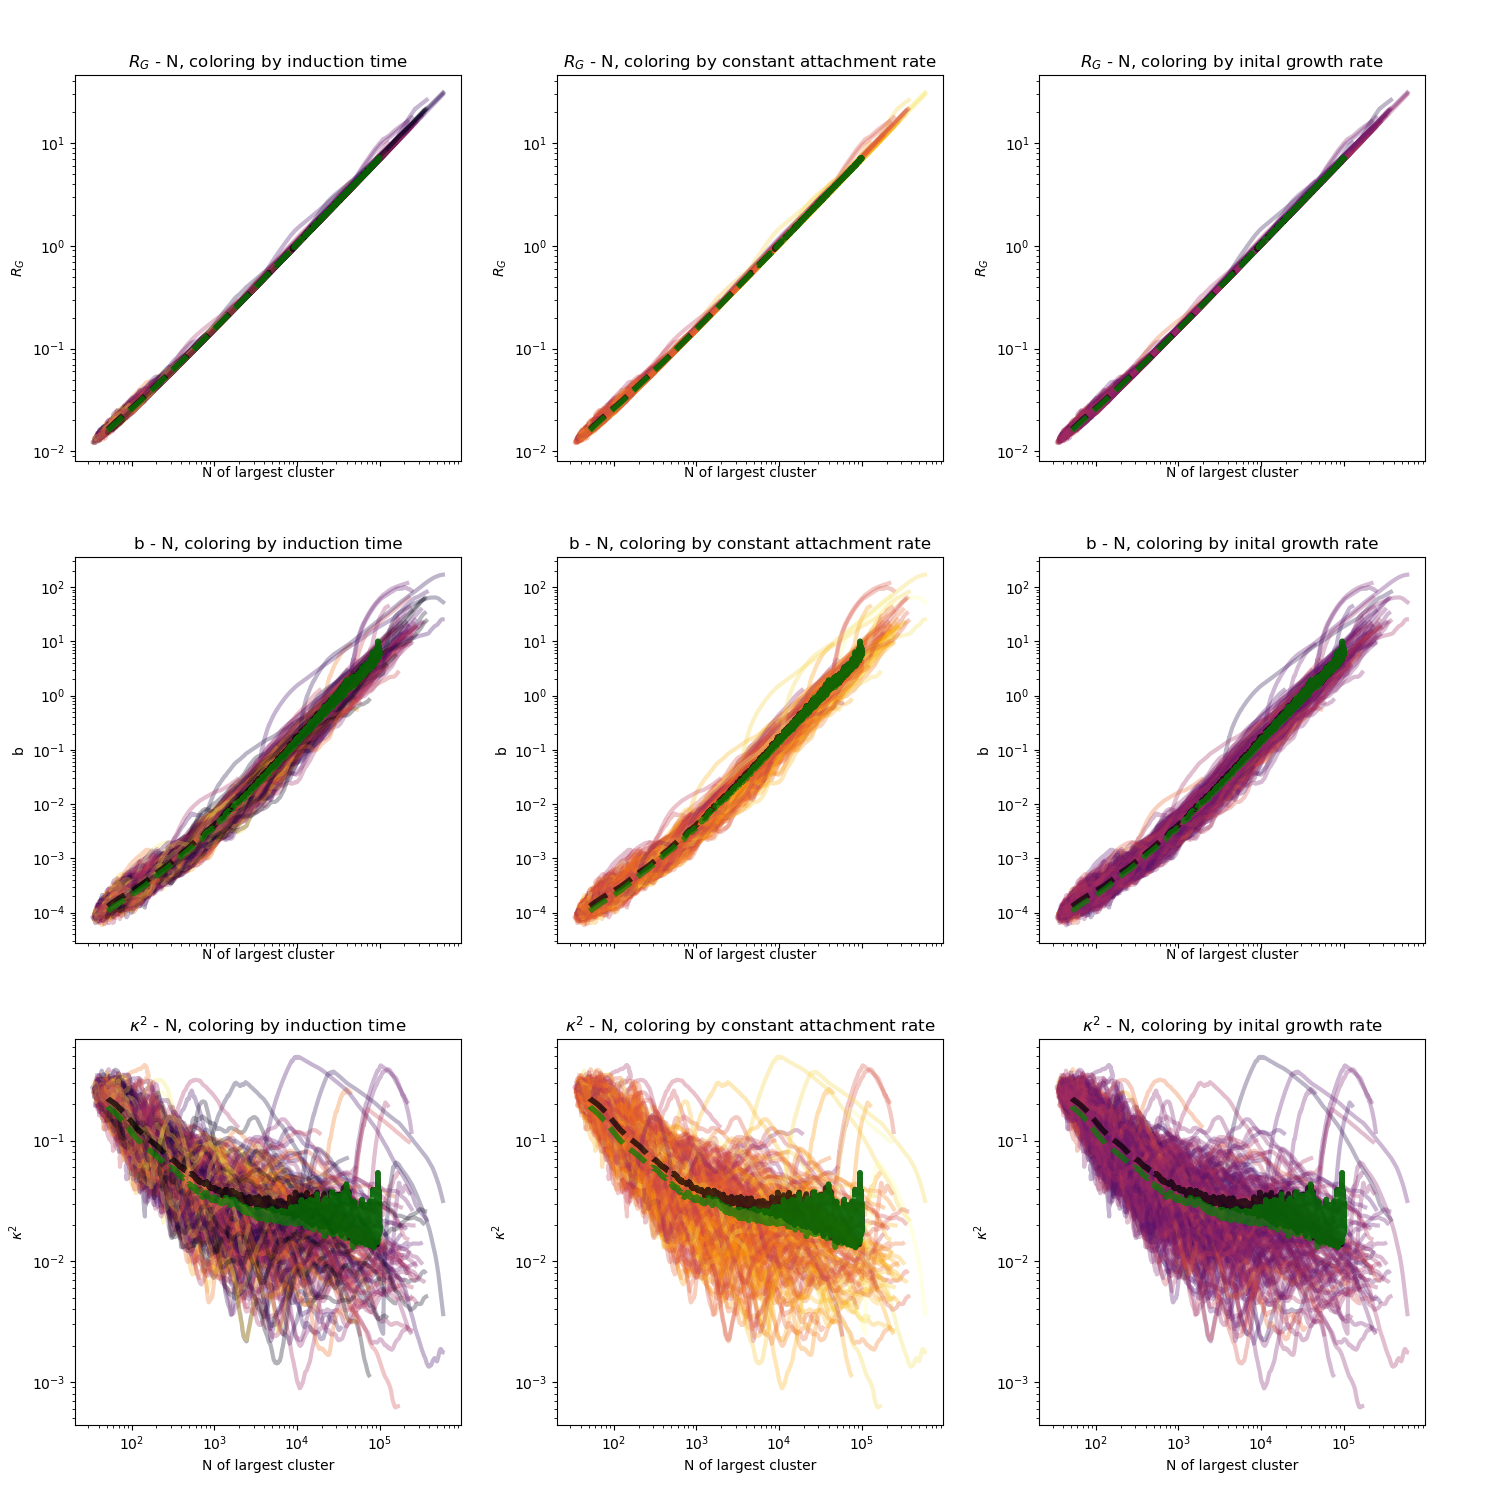
\includegraphics[width=0.8 \linewidth]{Series_534_corrolation.png}
\caption[Tensor of gyration measurements from production data]{Overview of the shape descriptors radius of gyration ($R_G$), asphericity (b) and anisotropy ($\kappa^2$), depending on the size of the cluster are shown. The coloring indicates the scalar quantities induction time, constant attachment rate and initial growth rate. Further a smoothed arithmetic mean and median are included in black and green respectively.}
\label{fig:tog_overview}
\end{figure}

From the overview we get no obvious sign that there are any correlations between cluster shape and growth rates or between cluster shape and the induction time. Because of that no deeper analysis is done, but instead we conclude that by this superficial analysis we cannot relate the shape descriptors to the cluster growth. Also a similar approach for the three scalar quantities that describe the growth process has been done, but neither showing significant correlations.\\  

Nevertheless from the calculated means, especially for the anisotropy $\kappa^2$, we can see that up to a size of about 1000 particles the clusters become more spherical while at higher particle numbers this tendency towards a sphere comes to an halt. This could be explained for example by the fact that the clusters always exhibit crystal faces leading to some unavoidable asphericity. An other explanation could be that the attachement rate for one crystal face might be higher than for an other, as this also would lead to unspherical growth. But as the clusters are rather close to a sphere, the attachemnt rate would also not vary much between the different crystal faces. It also has been observed that very large single crystals of a few hundred thousand particles may only form at volume fractions of $\eta = 53.2 \%$. At higher volume fractions domains form as it seems that heterogenous nucleation takes place close to the surface of the cluster, leading to new crystal orientations that are included into the crystal.\\


\section{Nucleation time dilemma}
\label{sec:nucleation_times}
To calculate induction times or average nucleation times, we will require a definition of when a crystal is called nucleated. This means we have to define the point at which a cluster is not merely an unstable fluctuation in the liquid anymore, but instead becomes a stable crystalline solid.\\
Many definitions can and have been used used for htis purpose. For example a cluster can be defined as crystalline soon as it surpasse the CNT's critical size or a multiple of it. One can also use a committer analysis to find the size where a crytallite keeps growing with a 50:50 chance. Also often apllied is the method to rewind a trajectory with a stable crystal back to the point where the cluster's size vanishes. A further approach is to fit the growth during later times and extrapolate it to the time when the cluster vanishes.\\

All these definitions differ only by a delay $\Delta_{\tau}$ which is a distribution holding the information of how long it takes for varying clusters to pass from the first criterion to the next.\\
For example we can take as a first point the time when a cluster, known to crystallize at later times, is not distinguishable from any other structural fluctuation in the liquid i.e. when the size of the cluster is below some threshold given by the size of clusters regularly present in a given volume.\\
The second point we can set by either the critical size of CNT or by some other criterion when we are sure that the cluster has stabilized and will only continue to grow.\\
At the first of these two points, the fluctuation leading to the crystallization occurs but it would not be possible to tell yet if this precursor melts or continues to grow, while at the second point the crystal is stable. For this reason the first might be called a precursor nucleation and the second crystal nucleation. Between these two points we find the time difference to be the time it takes for the precursors to form a stable crystal. This includes also that some precursors might loiter for awhile before forming the stable phase, while others pass this gap rather directly.\\

When calculating a mean induction time, the delay $\Delta_{\tau}$ propagates also to the final result and as it is a stochastic distribution also its higher moments are propagated leading to a smaller precision. After all this means that the induction time depends directly on the definition of crystallization and they are only roughly comparable. In \autoref{fig:induction_distributions} three distributions with varying definitions for the induction time are visualized.

\begin{figure}[!h]
\centering
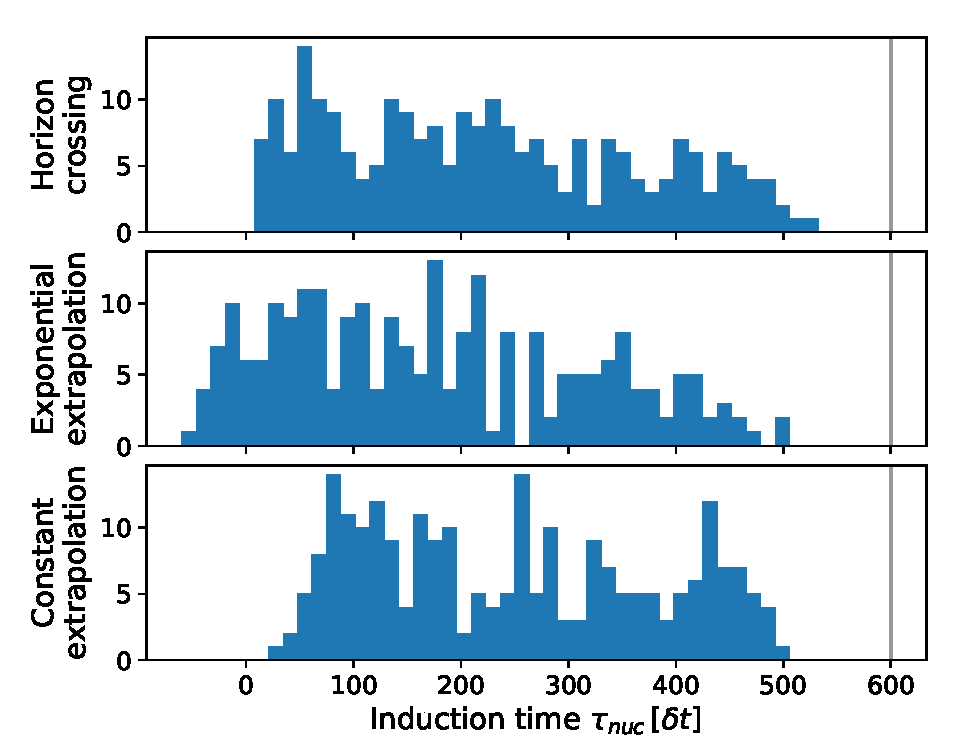
\includegraphics[width=0.6 \linewidth]{varying_induction_time.pdf}
\caption[Comparison of different definitions for the induction time]{Induction time distribution obtained by different definitions. While the two methods using extrapolation seem to have the two effects of smearing the signal as well as shifting them, the method of defining the nucleation as the time when the largest cluster is last below the horizon of fluctuations seems to return the most accurate and precise distribution. The final simulation time is marked by the grey line. As clusters require some time to clearly be recognized as crystals, no nucleation events are seen towards the end of the simulation interval. To counteract this we truncate the distribution in the analysis such it does not introduce a bias on the final result.}
\label{fig:induction_distributions}
\end{figure}

The three methods explicitly used here are given by the following:
\begin{description}
\item[Horizon crossing]{\hfill \\The time of nucleation is obtained by following the trajectory of the largest cluster within a nucleated system back to the point where it last crossed the average largest cluster of the metastable fluid. The name horizon crossing refers to the idea that fluctuations of the largest cluster are mostly independent, as the largest cluster is not fixed in the box, but fluctuations at different locations contribute. Only extraordinary large fluctuations will be seen for a prolonged periods of time and therefore will lead to correlated fluctuations of the largest cluster size. The crossing of the trajectory below this horizon, where it does not describe a distinct cluster anymore, is meant by the name.}

\item[Exponential extrapolation]{\hfill \\For this method an exponential growth is fitted to the largest cluster data up to N<500. Extrapolating to smaller times makes it possible to evaluate when the exponential function crossed 10 particles, which is then taken as the induction time. The method tends to find negative induction times that are not physical, but only an artifact of the method.}

\item[Constant extrapolation]{\hfill \\The name refers to the constant attachment rate found at later times for the cluster growth. It can be extrapolated to earlier times until the cluster completely vanishes. As the constant attachment rate is higher than the initial growth rate this method returns too large induction times.}
\end{description}

As can be seen the horizon crossing method returns a rather smooth distribution that also roughly can be approximated by an exponential decay that is expected for a constant nucleation rate as is shown in \autoref{sec:induction_time_expectation}.\\


\section{Induction time by exponential distribution assumption}
\label{sec:induction_times}
\todo{Some of this intorduction stuff may better fit into comparison to real world?}\\

Nucleation rates for the meatstable hard sphere fluid have been measured on the experimental as well as on the theoretical side, but with a large discrepancy as discussed in \autoref{sec:comparison}. The employed procedures and definitions also vary but not to a point to explain the discrepancy so far. The differences mostly originate from the kind of accessible system and information. While the experimentalists often have access to very large systems but without knowing all positions at all times, theorists mostly have smaller systems in numerical simulations but with the advantage of being able to access all particle positions and in case of MD simulations their velocities as well.\\
On the experimental side light scattering and optical methods are mostly employed to measure the structural properties of the probe, on the theoretical side different cluster finding algorithms are used.\\
While experimentalists may define an induction time by how long it takes for a quenched system to reach some level of overall crystallinity, theorists have often used simple approaches like the average time to nucleation for a couple of trajectories to measure their induction times for example by Filion et al. 2010\cite{Filion2010a} \todo{cite it here or not? It not such a positive statement}. This method requires the theorist to wait for all trajectories of an ensemble to show nucleation, what renders it very unsuitable for systems at low volume fractions where the induction time increases steeply.\\

To circumvent this problem we will define the nucleation rate in the following differently without requiring all simulations to nucleate. In fact we can also show that the uncertainty of the induction time obtained from the data is not significantly reduced anymore for measurements longer than the mean induction time.

\subsection{CNT expectation of the induction time distribution}
\label{sec:induction_time_expectation}
In \autoref{sec:CNT} we introduced classical nucleation theory and its constant nucleation rate depending on the barrier height in the free energy landscape. Even if there are signs that CNT is not appropriate for describing nucleation process completly, we will use its prediction of a constant nucleation rate as an assumption to define a constant scalar nucleation rate as well which can be compared to other literature values.\\

As mentioned before, in the discussion of the system sizes (\autoref{sec:system_choice}), the induction time of a system depends on the volume under consideration and for this reason it is commonly defined as a nucleation rate density $\kappa$. By using the diffusion time $\tau_L = D_L^{-1}$ as a unit of time furthermore makes the comparsion to other systems with faster or slower dynamics possible.\\

Considering a set of $m$ simulations at a given volume fraction, we can describe the total system as a sum of $m$ subvolumes, each of size $V_{box}$.  Further we can define the number of boxes in which a nucleation occurred as $n(t)$ and exclude these from the further simulation.\\

In this case the total nucleation rate $ \dot{n} $ can be written by \autoref{eqn:nuc_rate} from which in the continuous limit of an infinite number of subvolumes we can deduce the expected induction rate.

\begin{align}
\label{eqn:nuc_rate}
\dot{n} &= (m - n(t))V_{box}k\\
\Leftrightarrow \quad \!\frac{\dot{n}}{m} &= \left(1 - \frac{n(t)}{m}\right) V_{box}k \nonumber\\
 &  \text{in the limit } m \rightarrow \infty \nonumber\\
\Leftrightarrow \frac{n(t)}{m} &= 1 - \exp\left( -V_{box} k t \right)\\
 &  \text{defining } \tau = (V_{box} k)^{-1} \nonumber\\
\label{eqn:nuc_rate_result}
\Leftrightarrow \frac{\dot{n}(t)}{m} &= \frac{1}{\tau} \exp\left( \frac{-t}{\tau} \right) 
\end{align}

The final result in \autoref{eqn:nuc_rate_result} is the well known stochastic exponential distribution. As the expectation value of the exponential distribution is given by its parameter $\tau$, the common approach of using the mean induction time when all simulations have nucleated yields an accurate result and precision can be obtained by taking a large number of simulations.

\subsection{Maximum likelihood estimator of the induction time}
\label{sec:ml_estimator}
In case the simulation time is not accessible we instead will have to deal with truncated exponential distributions. For this we can use maximum likelihood (ML) estimators. The derivation follows the one by Deemer and Votaw 1955\cite{Deemer1955}.\\

Maximum likelihood estimators are based on the idea that we can write down the expression of the total probability called likelihood $\mathcal{L}$ for a given set of measurements $x_i$ depending on parameters of the assumed underlying distribution. For the exponential distribution, parameterized by the characteristic decay rate $\kappa$, it is given by

\begin{align}
\label{eqn:exponential_product}
\mathcal{L}(\kappa) = \prod_{i=1}^N p(x_i) = \prod_{i=1}^N \kappa^N \exp\left( - \kappa x_i \right ) \; \text{.}
\end{align}

We continue by find the maximum of this product. To simplify it and also to evade overflow problems on floating point machines, the logarithm of the likelihood is used and maximized yielding the same parameters because the logarithm is a monotonic function and thus does not shift the extrema.\\
The maximum probability can then be found by usual means of analysis executed in \autoref{eqn:exponential_maximization} - \autoref{eqn:exponential_maximization_end}.

\begin{align}
\label{eqn:exponential_maximization}
& 0 \stackrel{!}{=} \left. \frac{\partial \log (\mathcal{L})}{\partial \kappa} \right|_{\kappa=\hat{\kappa}}\\
\Leftrightarrow \qquad  &0 = \left. \frac{\partial}{\partial \kappa} \left( N \log(\kappa) - \kappa \sum_{i=1}^N t_i \right)  \right|_{\kappa=\hat{\kappa}} \\
\Leftrightarrow \qquad &0 = \frac{N}{\hat{\kappa}} - \sum_{i=1}^N t_i \\
\label{eqn:exponential_maximization_end}
\Leftrightarrow  \qquad & \!\!\!\!\!\!\!\!\: \hat{\kappa}^{-1} = \frac{1}{N} \sum_{i=1}^N t_i  
\end{align}

By this we have found that the maximum likelihood estimator of $\kappa$, for a set of samples drawn from an exponential distribution, is given by the inverse arithmetic mean of the samples. This result is neither new nor surprising but is shown to illustrate how the method of maximum likelihood works. In the following we then show how to handle censored and truncated distributions by the maximum likelihood method.\\
Both distributions refer to sets of samples that are incomplete in the sense that they only include samples up to some threshold $t_i < T$, but while in the case of truncated distributions the number of samples larger than this threshold is unknown, for the censored distribution it is known. Taking the example of time consuming nucleation events in computer simulations we are in the case of censored distributions, as the total number of boxes is known but the simulation is just stopped at some point without all boxes having had a nucleation event. The probability of an event later than the censoring time $T$ is given by
\begin{equation}
\label{eqn:prob_t_larger_T}
p(t_i>T) = \int_T^{\infty} \kappa \exp(-\kappa t) dt = \exp(-\kappa t) \; \text{.}
\end{equation}
Therefore we can write the complete probability distribution as
\begin{align}
\label{eqn:pdf_censored}
f(t) = 
\begin{cases}
\kappa \exp(-\kappa t) & t < T\\
\exp(-\kappa T) & t \geq T\\ 
\end{cases} \; \text{.}
\end{align}


In the simulation we can then split up the number of boxes $N$, into $n$ boxes where a nucleation event was found, and $m = N -n$ others where no nucleation event was spotted during the simulation time $T$.\\
Further we have to account for the fact that the samples without distinct times are indistinguishable. This is done by weighting them with the number of possible permutations which are calculated in the binomial prefactor $\binom{N}{m}$. The whole expression for the likelihood function $\mathcal{L}(\kappa)$ then is given by \autoref{eqn:ml_censored_exponential} and the extremum of it is evaluated in the subsequent reformulations.

\begin{align}
\label{eqn:ml_censored_exponential} 
\mathcal{L}(\kappa) & = \left. \binom{N}{m} \;  \kappa^n \; \exp(- \kappa \sum_{i=1}^n t_i) \;  \exp(-\kappa T)^m \quad \right| \left.\frac{\partial \log ( ... )}{\partial \kappa} \right|_{\kappa=\hat{\kappa}} \\
\Leftrightarrow \quad\log ( \mathcal{L}(\kappa)) & = \left.\log\binom{N}{m}  + n \log ( \kappa) - \kappa \sum_{i=1}^n t_i - m \kappa T \quad \right| \left. \frac{\partial(...)}{\partial \kappa} \right|_{\kappa=\hat{\kappa}} \\
\Leftrightarrow \:\! \frac{\partial \log ( \mathcal{L}(\kappa))}{\partial \kappa} & = \left. \frac{n}{ \kappa} - \sum_{i=1}^n t_i - m  T \quad \right|_{\kappa=\hat{\kappa}}\\ 
 & \; \; \, \vrule
  \begin{aligned}[t]
      \raisebox{0.9cm}{ \makebox[0.1cm]{}} \raisebox{-0.5cm}{ \makebox[0.5cm]{}}  \text{with } \frac{\partial \log ( \mathcal{L}(\hat{\kappa})  )}{\partial \kappa}  \stackrel{!}{=} 0  \\
  \end{aligned} \nonumber\\
\Leftrightarrow \qquad\qquad \;\; \:\! 0 &= \frac{n}{ \hat{\kappa}} - \sum_{i=1}^n t_i - m  T \quad\\
\label{eqn:ml_censored_exponential_final}
 \Leftrightarrow \qquad\quad  \;\: \hat{\kappa}^{-1} &= \frac{1}{n} \left(  \sum_{i=1}^n t_i + m T \right)
\end{align}


The final line \autoref{eqn:ml_censored_exponential_final} is the estimator of the decay rate of the censored exponential distribution. It is used for the estimation of induction times to compare with other published results in the next sections.

\subsection{Monte Carlo uncertainty estimation}
\label{sec:mc_uncertainty}
Having determined the estimator for the nucleation rate, the next question concerns its uncertainty i.e what is the distribution of $\hat{\kappa}$? While corresponding literature on analytic expressions for the distribution has been published for example by Chen and Bhattacharyya 1988\cite{Chen1988}, the complexity becomes inappropriate for the task at hand. Thus we will follow instead a Monte Carlo approach described for example in the book Numerical Recipes\cite{Press1992} to find the uncertainty of the estimator.\\

For this purpose we draw samples from an exponential distribution characterized by the estimator calculated from the actual simulation data. Afterwards the samples are censored by cutting off all elements larger than $T$ and calculate the corresponding estimator $\hat{\kappa}_{MC}$ for the Monte Carlo sample. From multiple such random sets we can create a histogram of estimates for $\hat{\kappa}$ that can be seen together with some exemplary random samples in \autoref{fig:mc_example}. As the distribution seems to incorporate only little higher moments, the standard deviation of the distribution is used as the estimators uncertainty $\sigma_{\hat{\kappa}}$.\\

\begin{figure}[ht]
%\begin{center}
\subfloat[Exponentially distributed random samples of size 500 with an exemplary censoring time of $T=\kappa^{-1}$]{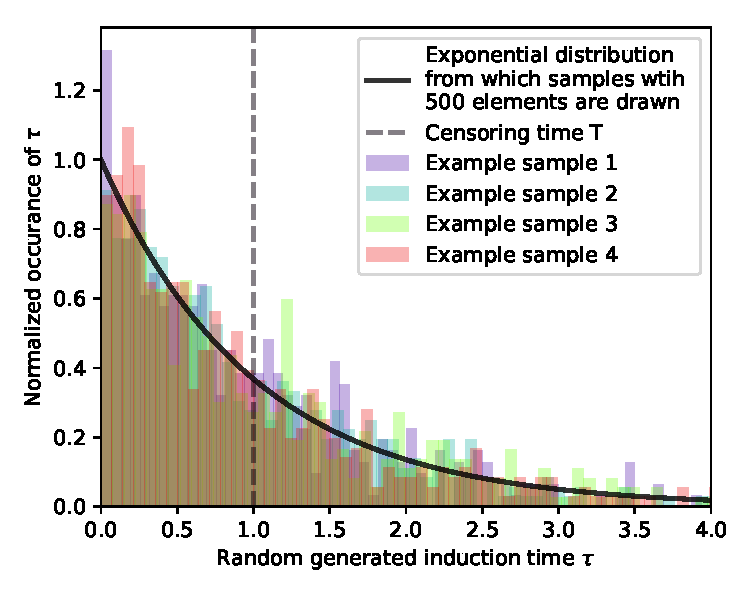
\includegraphics[width = 0.45 \textwidth]{mc_random_sample.pdf}} \hspace{0.5cm}
\subfloat[Distribution of $\hat{\kappa}$ for the previously generated MC samples. The distribution can be described mostly by mean and standard deviation as the number of estimates in the tails are small.]{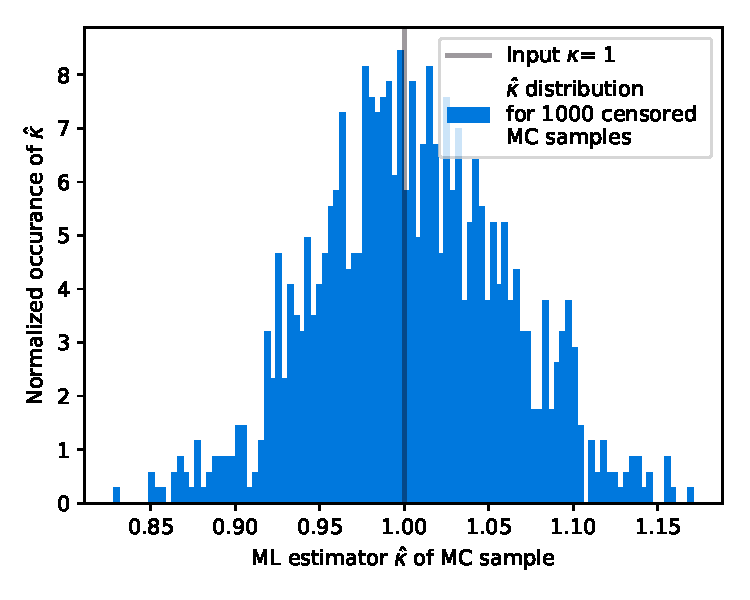
\includegraphics[width = 0.45 \textwidth]{k_estimator_distribution.pdf}}  
\caption[Monte Carlo uncertainty estimation example]{Exemplary samples for a given $\kappa$ as well as the distribution of estimates calculated from the random samples. The uncertainty on $\hat{\kappa}$ is approximated by the standard deviation of the distribution from the corresponding Monte Carlo analysis at a given $\kappa$.}
\label{fig:mc_example}
%\end{center}
\end{figure}
Concerning the uncertainty in detail we can ask how long a simulation should last to yield precise results. For this we can first look at the case where $1 \gg \kappa T$ corresponding to a simulation where all boxes showed a nucleation event. In this case we have seen before that $\hat{\kappa}^{-1} = \frac{1}{N} \sum_{i=1}^N t_i$. As we assume that the $t_i$'s are exponentially distributed we know that $\sigma_{t} = \kappa^{-1}$. Gaussian error propagation then results in
\begin{align}
\label{eqn:uncertainty_k_gg}
\frac{\sigma_{\hat{\kappa}}}{\hat{\kappa}} = \frac{1}{\sqrt{N}} \; \text{.}
\end{align}
%\begin{align}
%\label{eqn:uncertainty_k_gg}
%\frac{\sigma_{\kappa}}{\kappa} &=\frac{1}{\kappa} \sqrt{\sum_{i=1}^N \left( \frac{\partial \kappa}%{\partial t_i} \right)^2 \sigma_{t_i}^2 }\\ 
%& \; \; \, \vrule
%  \begin{aligned}[t]
%  \raisebox{0.9cm}{ \makebox[1cm]{}} \text{with }  \frac{\partial \kappa}{\partial t_i} &= %\frac{\partial}{\partial t_i} \left( N \left( \sum_{i=1}^N t_i \right)^{-1} \right)\\
%  &= -N\left( \sum_{i=1}^N t_i \right)^{-2}  = \frac{\kappa^2}{N} \; \text{,} \\
% \raisebox{-0.4cm}{ \makebox[1cm]{}} \text{and } \sigma_{t} &= \kappa^{-1}
%  \end{aligned} \nonumber\\
% &= \frac{1}{\kappa} \sqrt{ N \left( \frac{\kappa^2}{N}\right)^{2} \kappa^{-2} } \\
% &= \frac{1}{\sqrt{N}}
%\end{align}
%\todo{Is das eine Tautologie!?}
Similarly we can take the limit of $1 \ll \kappa T$ which is the case when the mean nucleation time is much larger than the simulation time and therefore only a small fraction of the boxes hosted a nucleation event. In this case we can expand the estimator in the fraction of nucleated trajectories $\frac{n}{N}$ to find $\hat{\kappa} \approx \frac{n}{N} \frac{1}{T}$. In this case the decrease of nucleation events due to the smaller not nucleated volume is not seen yet and the only information about the nucleation rate is obtained from the number of boxes with nucleations compared to the total number of boxes. As $n$ is Poisson distributed we know that $\sigma_n = \sqrt{n}$. Fixing N and T and using the expectation value of nucleations $n = N \hat{\kappa} T$, the Gaussian error propagation for the relative uncertainty is given in \autoref{eqn:uncertainty_k_ll}.
%\begin{align}
%\label{eqn:uncertainty_k_ll}
%\frac{\sigma_{\kappa}}{\kappa} &= \frac{1}{\kappa} \frac{\sqrt{n}}{NT} \nonumber\\
%&=\frac{\sqrt{N \kappa T}}{N T \kappa} \nonumber\\
%&=\frac{1}{\sqrt{N \kappa T}}
%\end{align}
\begin{align}
\label{eqn:uncertainty_k_ll}
\frac{\sigma_{\hat{\kappa}}}{\hat{\kappa}} = \frac{1}{\hat{\kappa}} \frac{\sqrt{n}}{NT} =\frac{\sqrt{N \hat{\kappa} T}}{N T \hat{\kappa}} =\frac{1}{\sqrt{N \hat{\kappa} T}}
\end{align}
Finally we are also able to not only look at limits analytically, but also to approximate the relative uncertainty directly by means of the aforementioned Monte Carlo method. For this purpose the same procedure as before is used. The number of elements per sample is set consistently with the actual number of used simulations to 500 and to achieve good precision on the uncertainty, the standard deviation of 1000 samples is used. To compare the analytically derived limits of the uncertainty with the Monte Carlo results both are drawn into \autoref{fig:relative_uncertainty}.

\begin{figure}[ht]
\begin{center}
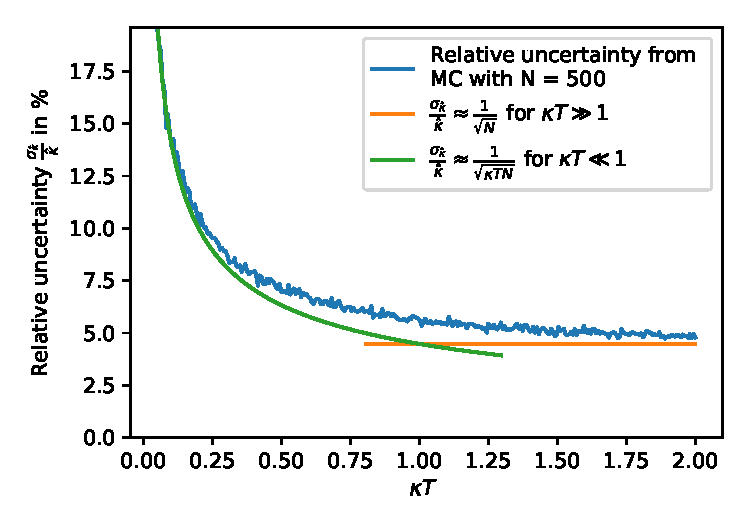
\includegraphics[width = 0.65 \textwidth]{rel_uncertainty_k.pdf}
\caption[Nucleation rate uncertainty depending on measurement time]{Relative uncertainty of the ML estimator for varying $\kappa T$. The x scale is chosen dimensionless such that it indicates the simulation time in comparison to the characteristic nucleation time.}
\label{fig:relative_uncertainty}
\end{center}
\end{figure}

We find that for the limits of $\kappa T \ll 1$ as well as $\kappa T \gg 1$, Monte Carlo and analytical results are in good accordance while in between the analytical limits only can be used as a rough estimate.\\

What can be seen from \autoref{fig:relative_uncertainty} is that the uncertainty of the estimation drops sharply until about half of the characteristic induction time, after which it only obtains little more precision. This is not surprising as the nucleation times contain the rate and more nucleation events occur at the beginning while long simulation times only add little further information. Thus simulating until all boxes hosted a nucleation event is only necessary if one wants to use the simpler arithmetic mean of the induction times as the setimator, or if any other constraints make it necessary to reach crystallization of all boxes.

\section{Nucleation rate comparison}
\label{sec:nucleation_rates}
Finally we are able to evaluate the induction time distribution to find the rates given in \autoref{fig:nucleation_comparison}.

\begin{figure}[h!]
\centering
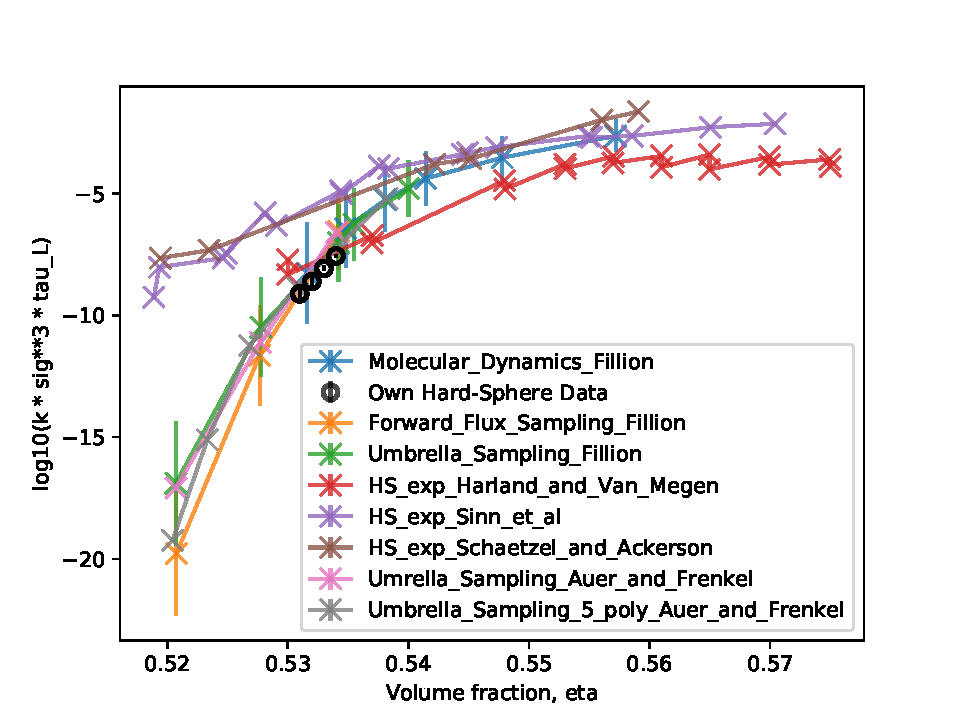
\includegraphics[width=0.6 \linewidth]{nucleation_rate_comparison.pdf}
\caption[Nucleation rate comparison with literature values]{Experimental and theoretical examples of nucleation rates in the hard sphere system at different volume fractions from the literature \todo{citations and/or other data}, to compare with the own measured data points.}
\label{fig:nucleation_comparison}
\end{figure}

From the diagram we can state that our measurements confirm the previous simulation results, that still stand against the experimentally found ones. Further the results are calculated together with their statistical uncertainty which is mostly visible for the data point at $\eta = 53.1 \%$. It is also indicated for the others but due to the logarithmic scaling the uncertainty is almost not visible.\\
While uncertainties in the literature are often just very roughly given, the here presented method makes
it possible to quantify the statistical uncertainty of the rates and the large number of simulations give us high precision in comparison to rates elsewhere found. 

\section{Memory kernels of nucleating ensemble}
\label{sec:memory_kernels}
The approach by Hugues Meyer et al. 2019\cite{Meyer2019a}, to calculate memory kernels from an ensemble of trajectories, is used on the data discussed in the previous sections as well as on trajectories of a system characterized in \autoref{tab:system_16k_mem}. The second system is used because the first ensemble was neither simulated up to the point where most boxes contained a stable cluster nor until the boxes were fully crystallized as the transition width is large and takes very long simulations to fill up the large box. The second system's parameters are chosen to fulfill both objections.\\

\begin{table}[ht]
\centering
\begin{tabular}{c|c}
Parameter & Value \\ \hline
N & 16384 \\
eq\_steps/particle & 5000 \\
pr\_steps/particle & 200000 \\
$\eta_i$ & 45.0 \% \\
$\eta_f$ & 53.4 \% \\
\end{tabular}
\caption[Simulation parameters of data production system with 16384 particles]{Input parameters of simulations on the NEMO HPC cluster. The large number of production steps is chosen, together with the final volume fraction $\eta_f$, in a way to simulate nucleation and full crystallization of the boxs in almost all cases as can be seen in the top diagram of \autoref{fig:cluster_growth_example}. Furthermore the small box size leads to a small transition width $\Delta$ of about $150 \delta t$ corresponding closely to the width of the memory kernel, as lately shown by Meyer et al. 2021\cite{Meyer2021}.} 
\label{tab:system_16k_mem}
\end{table}

Still the memory kernel of the large system has been calculated but except of the Markovian contribution only little of the memory kernel was visibible, indicating that the sample is not sufficently long or that the largest cluster is not an appropriate observable for nucleations in large systems.\\

To compare the memory kernel with direct measurements of the observable the evolution of the ensemble is depicted in the top of \autoref{fig:cluster_growth_example}. The trajectories have been normalized by the number of particles in the box and some statistical properties likes percentiles and arithmetic mean are also shown as the large number of trajectories otherwise makes it hard to distinguish the actual density of lines at some points. At the bottom of the figure the share of trajectories at different stages of the nucleation process is identfied. For this it is assumed that trajectories below an normalized largest cluster of 0.1 can be identified as not nucleated, such trajectories above 0.5 as fully crystallized and all trajectories in between as in the crystallization process.\\

\begin{figure}[ht]
\centering
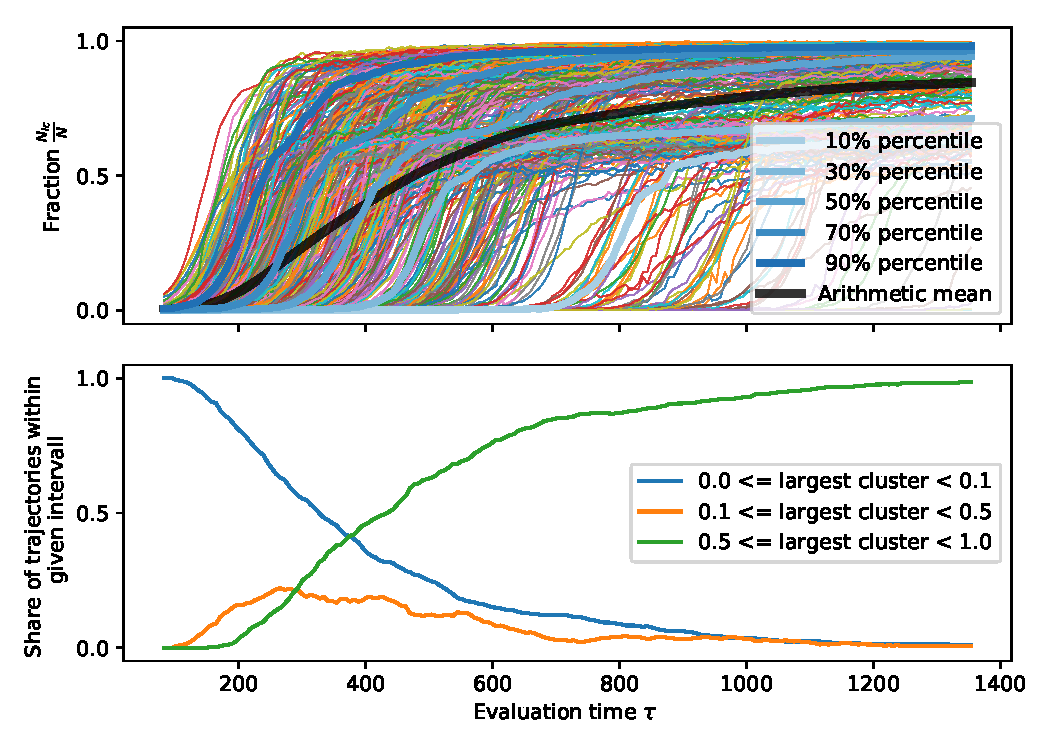
\includegraphics[width=0.7 \linewidth]{cluster_growth_quantities.pdf}
\caption[Largest cluster trajectories of small system with percentiles and average]{Top: Normalized trajectories of largest cluster with percentiles and arithmetic mean indicated. It can be observed that a fraction of the trajectories nucleates in more than one step where at first only about 60\% of the box is filled by the crystal and at later times they sometimes crystallize further until almost the complete box is filled by the solid phase. From \autoref{eqn:solid_fraction_result} we would expect an equilibrium solid fraction of 80\% by volume, closely corresponding to the expected solid fraction by particles.\\
Bottom: Fraction of trajectories within intervals chosen to identify nucleated trajectories, momentary growing trajectories and fully nucleated trajectories. As the growth process is much faster than the distribution of nucleations, the orange curve roughly resembles the derivative of the other two curves.}
\label{fig:cluster_growth_example}
\end{figure}

While for the large system only little of the crystallites reached the box boundaries in this latter we see that almost all clusters fill the whole box at the end of the simulation.\\
Further as there is no clear analysis yet on how the direct quantities and the memory kernel are related, the subdivision is an approach to show direct observables that possibly are related to properties of the memory kernel.\\

We see in on the left of \autoref{fig:memory_kernel}, that the shape of a memory kernel slice at some reference time is rather simple. For this reason we use a Gaussian fit to approximate the width and amplitude of the kernel. For this purpose we neglect the Markovian part of the kernel at around $t_1-t_2 \approx 0$. To validate the fit results we further use the FWHM, where the maximum is determined by the mean value of the peak's crest.\\
As the properly normalized results for both methods are in good agreement, we can conclude that the shape of the memory kernel in this case is mostly defined by a width and an amplitude over time which are depicted on the right of \autoref{fig:memory_kernel}.\\

\begin{figure}[ht]
\begin{center}
\subfloat[Slice through memory kernel at the given reference time. With the data the excluded Markovian part of the kernel is depicted. Further the full width at half maximum (FWHM) is shown as a first measure of the kernel width as well as a Gaussian fit. The FWHM is normalized to the value of a corresponding Gaussian curve.]{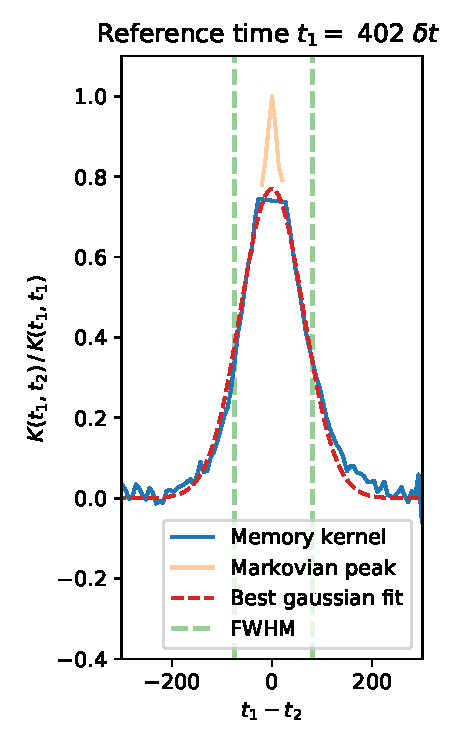
\includegraphics[width=0.37 \linewidth]{example_memory_kernel.pdf}} \hspace{0.5cm}
\subfloat[Top: Width of the memory kernel slices from FWHM and Gaussian fit. The FWHM is normalized to the value of a corresponding Gaussian curve.
Bottom: Amplitude of the memory kernel slice on the one hand by using the mean value of the data around the maximum and on the other hand by using the amplitude derived from the best Gaussian fit. The amplitude derived from the maximum value is normalized to the value of a corresponding Gaussian curve.]{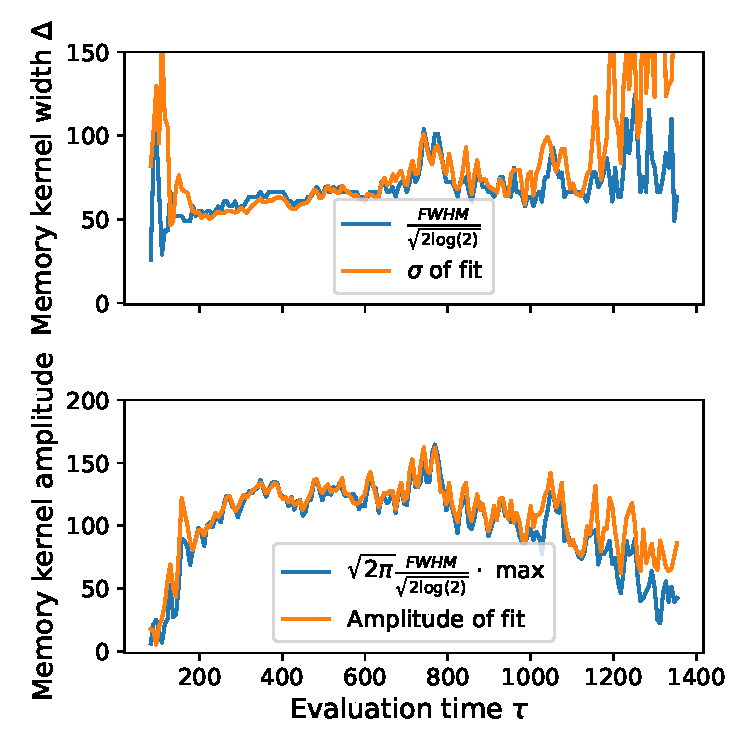
\includegraphics[width=0.59 \linewidth]{memory_kernel_shape.pdf}}
\caption[Width and amplitude of memory kernel with example slice]{Example memory kernel together with width and amplitude depending on time.}
\label{fig:memory_kernel}
\end{center}
\end{figure}

The width of the memory kernel sections are mostly constant over the whole measurement with the exception that it becomes very noisy at the end.\\
The amplitude in comparison increases at the beginning, remains over a prolonged period of time constant and then declines towards the end of the measurement.\\
As published by Meyer et al. 2021\cite{Meyer2021}, the width of the memory kernel seems to depend on the phase transition time. Because for the hard sphere system the transition width is mostly given by the arbitrarily chosen box size, the dependence is possibly only an artifact with other memory effects buried beneath.\\ 

To seperate these memory effects one could generate trajectories with a purely Markovian approach, like Brownian dynamics, with corresponding characteristic properties. Then comparing the memory kernels of the purely Markovian ensemble with the a priori non Markovian hard sphere ensemble may help to distinguish memory effects due to the system size from those related to the dynamics of the fluid.\\

An other approach would be to use the committer probability of the largest cluster as an observable, as it would not include a direct system size dependence and by itself is already bounded between zero and one, which is a requirement for the memory kernel analysis.
